
Learning from interactions with users is ubiquitous in modern customer-facing platforms, from product recommendations to web search to content selection to fine-tuning user interfaces. Many platforms purposefully implement \emph{exploration}: making potentially suboptimal choices for the sake of acquiring new information.
Online platforms routinely deploy A/B tests, and are increasingly adopting  more sophisticated exploration methodologies based on \emph{multi-armed bandits}, a standard and well-studied framework for exploration and making decisions under uncertainty
\citep{Gittins-book11,Bubeck-survey12,slivkins-MABbook,LS19bandit-book}.

%~\cite{KohaviAB-2015,KohaviLSH09}

In this paper, we initiate a study of the interplay between \exploration and \competition. Platforms that engage in exploration typically need to compete against one another; most importantly, they compete for users. This creates a tension:
%between \exploration and \competition.
while exploration may be essential for improving the service tomorrow, it may degrade quality and make users leave \emph{today}, in which case there will be less users to learn from. This may further degrade the platform's performance relative to competitors who keep learning and improving from \emph{their} users, and so forth. Taken to the extreme, such dynamics may create a ``death spiral" effect when the vast majority of customers eventually switch to competitors. Users therefore serve three distinct roles: they are customers that generate revenue, they are sources of data for learning, and they are self-interested agents who choose among the competing systems.

The main high-level question that we focus on in this paper is:
\begin{align}\label{eq:main-Q}
\textbf{How does competition incentivize the adoption of better exploration algorithms?}
\end{align}

\noindent This translates into a number of more concrete questions. While it is commonly assumed that better technology always helps, is this so under competition? Does increased competition lead to higher consumer welfare? How significant are ``data feedback loops" --- when more data leads to more users, which leads to even more data, etc. --- and how they relate to the anti-trust considerations? Finding formalizations that admit meaningful answers is a major part of the overall challenge.




To answer these questions, we study complex interactions between platforms' learning dynamics and users' self-interested behavior. The choice of a particular technology (exploration algorithm) is no longer an abstract, static choice with a predetermined outcome for the platform. Instead, we model the algorithms explicitly, and investigate how they play out in competition over an extended period of time.


%\footnote{This is a fundamental question which is part of a larger policy discussion around whether data can serve as an indirect network effect and lead to similar ``market tipping" results as is standard in the literature on competition in markets with network effects (see \cite{jullien2019economics} for a policy oriented discussion of this).}

% the extent to which the game between the two principals is competitive
% degree of innovation that these models incentivize.
% the extent to which agents make rational decisions


%\subsection{Our model}
%\label{sec:intro-model}

\subsection{Our model: competing bandits}
\label{sec:intro-model}

%We investigate these questions with
\xhdr{Competition game.} We consider a stylized duopoly model where two firms commit to exploration strategies and compete for a stream of consumers. We define a game in which two firms (\emph{principals}) simultaneously engage in exploration and compete for users (\emph{agents}). These two processes are interlinked, as exploration decisions are experienced by users and informed by their feedback. We need to specify several conceptual pieces: how the principals and agents interact, what is the machine learning problem faced by each principal, and what is the information structure. Each piece can get rather complicated in isolation, let alone jointly, so we strive for simplicity. Thus, the key features of our model are as follows:

\begin{itemize}

\item A new agent arrives in each round $t=1,2, \ldots$, and chooses among the two principals. The principal chooses an action (\eg a list of web search results to show to the agent), the user experiences this action, and reports a reward. All agents have the same ``decision rule" for choosing among the principals given the available information.

\item Each principal faces a basic and well-studied version of the multi-armed bandit problem: for each arriving agent, it chooses from a fixed set of actions  (a.k.a. \emph{arms}) and receives a reward drawn independently from a fixed distribution specific to this action. The reward distributions are initially unknown (but can be estimated over time from the data).

\item Principals simultaneously announce their bandit algorithms before round $1$, and cannot change them afterwards.  Each principal's objective is to maximize its market share (the fraction of users choosing this principal). Each principal only observes agents that chose this principal.
%, but may have access to each platforms' reputation score (more on this in    Section~\ref{sec:intro-discussion}).
\end{itemize}

\noindent We investigate several model variants within this framework, where we vary agents' decision rule and/or give a first-mover advantage to one of the principals. In all variants, agents have little or no information about other agents' choices and rewards.

%We consider two model variants, which determine agents' decision rule and their information sets. In \emTheoryModel, there is a common Bayesian prior on the reward distributions. Agents do not receive any other information and choose between the principals using their knowledge of $t$ and the principals' algorithms. In \emExptsModel, agents have access to a reputation score for each principal, which is a sliding window average of the rewards experienced by previous agents that have visited this principal. The former variant used for the theoretical results, the latter for simulations.

\xhdr{Technology: multi-armed bandit algorithms.}
To flesh out \eqref{eq:main-Q}, let us elaborate what we mean by `better' bandit algorithms. In general, comparisons between bandit algorithms are rather subtle, as some algorithms may be better for some problem instances and/or time intervals, and worse for some others.

\gaedit{While our model allows for the firms to pick from an arbitrary set of algorithms}, we distinguish between three classes of bandit algorithms, based on the prevalent intuition in the area. The distinction concerns the way in which they resolve the fundamental tradeoff between  exploration and \emph{exploitation} (making optimal myopic decisions using the available data). \gaedit{This classification is important for interpreting the equilibrium algorithm choice of the firms as it allows for a ``low" to ``medium" to ``high" technology interpretation. We further use the classification to pick a representative algorithm from each class for our numerical experiments. Going from low to medium to high, these three classes are as follows:} \gadelete{Going from more primitive to more sophisticated, these three classes are as follows:}

\begin{itemize}
\item \emph{Greedy algorithms} that strive to maximize the reward for the next round given the available information. Thus, they always ``exploit" and never explicitly ``explore".

\item \emph{Exploration-separating algorithms}
 that separate exploration and exploitation: essentially, each round is dedicated to one and completely ignores the other.

\item \emph{Adaptive-exploration} algorithms that combine exploration and exploitation, and gradually sway the exploration choices towards more promising alternatives.
\end{itemize}

In isolation, \ie in the absence of competition, these classes are fairly well-understood. Greedy algorithms are terrible for a wide variety of problem instances, precisely because they never explore. Exploration-separated algorithms learn at a reasonable but mediocre rate across all problem instances. Adaptive-exploration algorithms are optimal in the worst case, and exponentially improve for ``easy" problem instances. Generally,  ``better" algorithms are better in the long run, but could be worse initially.

While we build on a vast and active research area, we present sufficient background in Appendix~\ref{app:bg} so as to keep this paper accessible to non-specialists.


\subsection{Our results}
\label{sec:intro-results}

We offer a mix of theoretical results and numerical simulations. We are mainly interested in qualitative differences between the three classes of algorithms in Section~\ref{sec:intro-model}. For numerical simulations, we pick one representative algorithm from each class. For theoretical results, we allow arbitrary algorithms and focus on asymptotic differences in the algorithms' performance.

\xhdr{Theoretical results.}
%We endow agents with Bayesian rationality, a common modeling approach for a theoretical investigation.
We consider a basic Bayesian model. We posit that agents have a common Bayesian prior on reward distributions, and know the principals' algorithms. For simplicity, agents do not receive any information about the previous agents' choices and rewards. Each agent knows the round (s)he arrives in, computes the Bayesian-expected reward for each principal, and use these two numbers to decide which principal to choose. We refer to this variant as the \emph{\TheoryModel}.

Our results depend crucially on the agents' decision rule.
\begin{itemize}

\item The most obvious decision rule maximizes the Bayesian-expected reward; we refer to it as \HardMax. We find that \HardMax is not conducive to adopting better algorithms: each principal's dominant strategy is to choose the greedy algorithm. Further, we show that \HardMax is very sensitive to tie-breaking: if the tie-breaking is probabilistically biased in favor of one principal, then this principal has a simple ``winning strategy" no matter what the other principal does.

\item We dilute the \HardMax agents with a small fraction of ``random agents" who choose a principal uniformly at random. We call this model \HardMaxRandom. We find that better algorithms help in a big way: a sufficiently better algorithm is guaranteed to win all non-random agents after an initial learning phase. However, there is a substantial caveat: one can defeat any algorithm by interleaving it with the greedy algorithm. This has two undesirable corollaries: a better algorithm may sometimes lose in competition, and a pure Nash equilibrium typically does not exist.

\item We further relax the decision rule so that the probability of choosing a given principal varies smoothly as a function of the difference between  principals' Bayesian-expected rewards; we call it \SoftMaxRandom. For this model, the ``better algorithm wins" result holds under much weaker assumptions on what constitutes a better algorithm. This is the most technical result of the paper. The competition in this setting is necessarily much more relaxed: typically, both principals attract approximately half of the agents as time goes by (but a better algorithm would attract slightly more).
\end{itemize}

All results extend to a much more general version of the multi-armed bandit problem in which the principal may observe additional feedback before and/or after each decision, as long as the feedback distribution does not change over time. In most results, principal's utility may depend on both the market share and agents' rewards.

\begin{figure}
\begin{center}
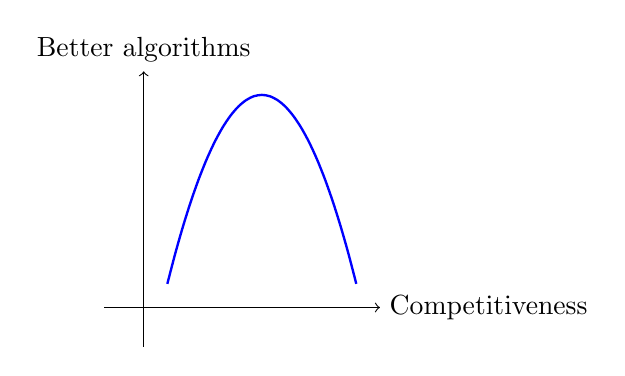
\begin{tikzpicture}
      \draw[->] (-.5,0) -- (3,0) node[right] {Competitiveness};
      \draw[->] (0,-.5) -- (0,3) node[above] {Better algorithms};
      \draw[scale=0.6,domain=0.5:4.5,smooth,variable=\x,blue, line width=0.3mm] plot ({\x},{4.5 - (\x - 2.5)^2});
      % \draw[scale=0.5,domain=-3:3,smooth,variable=\y,red]  plot ({\y*\y},{\y});
 \end{tikzpicture}

\caption{Inverted-U relationship between competitiveness and algorithms.}
\label{fig:inverted-U}
\end{center}
\end{figure}


\xhdr{Economic interpretation: the inverted-U relationship.}
Interpreting the adoption of better algorithms as ``innovation", our findings can be framed in terms of the inverted-U relationship between competition and innovation, as in Figure~\ref{fig:inverted-U}.%
\footnote{Here, ``innovation" refers to adoption of a better technology at a substantial R\&D expense to a given firm. It is not salient whether similar ideas and/or technologies already exist elsewhere. Adoption of exploration algorithms tends to require substantial R\&D effort in practice, even if the algorithms themselves are well-known in the research literature \citep[\eg see][]{DS-arxiv}.}
This is a well-established concept in the economics literature, dating back to \cite{Schumpeter-42}, whereby too little or too much competition is bad for innovation, but intermediate levels of competition tend to be better \citep[\eg][]{aghion2005competition,Vives-08}.

Our decision rules differ in terms of rationality: from fully rational decisions with \HardMax to relaxed rationality with \HardMaxRandom to an even more relaxed rationality with \SoftMaxRandom. The same distinctions also control the severity of competition between the principals: from cut-throat competition with \HardMax to a more relaxed competition with \HardMaxRandom, to an even more relaxed competition with \SoftMaxRandom. Indeed, with \HardMax you lose all customers as soon as you fall behind in performance, with \HardMaxRandom you get some small market share no matter what, and with \SoftMaxRandom you are further guaranteed a market share close to $\tfrac12$ as long as your performance is not much worse than the competition. The uniform choice among principals corresponds to no rationality and no competition. While agents' rationality and severity of competition are often modeled separately in the literature, it is not unusual to have them modeled with the same ``knob" \cite[\eg][]{Gabaix-16}.


We identify the inverted-U relationship driven by the rationality/competitiveness distinctions outlined above: from \HardMax to \HardMaxRandom to \SoftMaxRandom to \Uniform. We also find another, technically different, inverted-U relationship which zeroes in on the \HardMaxRandom model. We vary rationality/competitiveness inside this model, and track the marginal utility of switching to a better algorithm.

These inverted-U relationships are driven by different aspects in our model than the ones in the existing literature in economics. The latter focuses on the tradeoff between the R\&D costs and the benefits that the improved technology provides in the competition. In our case, the barriers for innovations arise entirely from the reputational consequences of exploration in competition, even in the absence of R\&D costs.


\xhdr{Numerical simulations.}
We consider a basic frequentist model. We posit that the agents observe signals about the principals' past performance, and base their decisions on these signals alone, without invoking any prior knowledge or beliefs. The performance signals are abstracted and aggregated as a scalar \emph{reputation score} for each principal, modeled as a sliding window average of its rewards. Thus, agents' decision rule depends only on the two reputation scores. We refer to this variant as the \emph{\ExptsModel}.%
%\footnote{In comparison, the theoretical results focus on another extreme, with Bayesian rationality and no performance signals.}

We refine and expand the theoretical results in several ways.

\begin{itemize}
\item We compare \HardMax and \HardMaxRandom decision rules. We find that the greedy algorithm often wins under \HardMax, with a strong evidence of the ``death spiral" effect mentioned earlier.
 As predicted by the theory, better algorithms prevail if the expected number of ``random" users is sufficiently large. However, this effect is negligible for smaller parameter values.

%\footnote{\asedit{Reputation scores already introduce some noise into users' choices. However, the amount of noise due to this channel is typically small, both in our simulations and in practice, because reputation signals average over many datapoints.}}

\item We investigate the first-mover advantage as a different channel to vary the intensity of competition: from the first-mover to simultaneous arrival to late-arriver. (We focus on the \HardMax decision rule.) We find that the first-mover is incentivized to choose a more advanced exploration algorithm, whereas the late-arriver is often incentivized to choose the ``greedy algorithm" (more so than under simultaneous arrival). Consumer welfare is higher under early/late arrival than under simultaneous entry. We frame these results in terms of an inverted-U relationship.


%\footnote{\asedit{We consider the ``permanent monopoly" scenario for comparison only, without presenting any findings. We just assume that a monopolist chooses the greedy algorithm, because it is easier to deploy in practice. Implicitly, users have no ``outside option": the service provided is an improvement over not having it (and therefore the monopolist is not incentivized to deploy better learning algorithms). This is plausible with free ad-supported platforms such as Yelp or Google.}}

\item We investigate the algorithms' performance ``in isolation", \ie without competition. We suggest a new performance measure to explain why the greedy algorithm is sometimes not the best strategy under high levels of competition.\footnote{Note the discrepancy with our theoretical results on \HardMax: there, the greedy algorithm is always the best strategy, mainly because it is aware of the Bayesian prior (whereas in the simulations the prior is not available).}
     We find that mean reputation -- arguably, the most natural performance measure ``in isolation" -- is sometimes \emph{not} a good predictor for the outcomes under competition.

\item We decompose the first-mover advantage into two distinct effects: free data to learn from (\emph{data advantage}), and a more definite, and possibly better reputation compared to an entrant (\emph{reputation advantage}). We run additional experiments so as to isolate and compare these two effects. We find that either effect alone leads to a significant advantage under competition. The data advantage is larger than reputation advantage when the incumbent commits to a more advanced bandit algorithm. Finally, we find an ``amplification effect" of the data advantage: even a small amount thereof gets amplified under competition, causing a large difference in eventual market shares.

\end{itemize}

\ascomment{One downside of the story above: we may need to explain why we didn't simulate \SoftMaxRandom.}

\ascomment{The xhdr below is basically from Guy, with some rewordings by Alex.}

\xhdr{Economic interpretation: network effects of data.}
Our model speaks to policy discussions on regulating data-intensive digital platforms \citep{furman2019unlocking, scott2019committee}, and particularly to the ongoing debate on the role of data in the digital economy. One fundamental question in this debate is whether data can serve a similar role as traditional ``network effects", creating scenarios when only one firm can function in the market \citep{Rysman09, jullien2019economics}.
%whereby, when these effects are present, in many cases only one firm can function in the market, leading to competition \emph{for} the market being more important than competition \emph{in} the market \citep{Rysman09, jullien2019economics}.
The death spiral/amplification effects mentioned above have a similar flavor as network effects: a relatively small amount of exploration (resp., data advantage)  gets amplified under competition and causes the firm to be starved of users (resp., take over most of the market).
%\gaedit{We further find that a small data advantage for one firm gets amplified under competition and leads to that firm taking the entire market, showing that data can provide a similar incumbency advantage as those provided by traditional network effects and can serve as a barrier to entry in online markets.}
A distinctive feature of our approach is that we explicitly model the learning problem of the firms and consider them deploying algorithms for solving this problem.  Thus, we do not explicitly model the network effects, but they arise endogenously from our setup.

Our results highlight that understanding the performance of learning algorithms in isolation does not necessarily translate to understanding their impact in competition, precisely due to the fact that competition leads to the endogenous generation of data observed by the firms. Approaches such as \citet{lambrecht2015can, bajari2018impact, varian2018artificial} argue that the diminishing returns to scale and scope of data in isolation mitigate such data feedback loops,
%as non-existent
but ignore the differences induced by learning in isolation versus under competition. Furthermore, explicitly incorporating the interaction between learning technology and data creation allows us to speak on how data advantages are characterized and amplified not only by data quantity, but also the increased data quality gathered by better learning algorithms.

\ascomment{"Econ interpretation" xhdrs fit incely in "our results", as opposed to a separate subsection. Because: we can explain the "inverted-U" stuff right after "theory", before we put the simulation results on the stack. And the "network effects" stuff goes nicely right after the numerical results, without a big subsection break.}



\subsection{Further discussion}
\label{sec:discussion}

\xhdr{Significance.}
Our theory takes a basic Bayesian approach, a standard perspective in economic theory, and discovers several strong asymptotic results. The numerical simulations provide a more nuanced and ``non-asymptotic" perspective. In essence, we look for substantial effects within relevant time scales. In fact, we start our investigation by determining what time scales are relevant in the context of our model.

\ascomment{The next para makes a point that seems important (to me). Is this point clear?}

Our study has a dual purpose: (i) shed light on real-world implications of some typical scenarios, and (ii) investigate the space of models for describing the real world. As an example to clarify the latter point, consider the \HardMax model with simultaneous entry. It is is not necessarily the most realistic model, but arguably the most natural one to study \emph{a priori}. However, our results elucidate the need for more refined models that allow for ``free exploration" (\eg via random agents or early entry).

\xhdr{Modeling.}
Our models are stylized in several important  respects. Firms compete only on the quality of service, rather than, say, pricing or the range of products. Agents are myopic: they do not worry about how their actions impact their future utility.\footnote{In particular, agents do not attempt to learn over time, to second-guess or game future agents, or to manipulate the principals' learning algorithms. This is arguably typical in practice, in part because one agent's influence tends to be relatively small.}  Various performance signals available to the users, from personal experience to word-of-mouth to consumer reports, are abstracted as persistent ``reputation scores", and further simplified to average performance over a time window. On the machine learning side, our setup is geared to distinguish between ``simple" vs. ``better" vs. ``smart" bandit algorithms; we are not interested in state-of-art algorithms for very realistic bandit settings.

We consider two extremes: a simple Bayesian model with full Bayesian rationality and no performance signals, and a simple frequentist model with reputation scores and no prior knowledge or beliefs. For the theoretical results, the ``no-performance-signals" assumption makes agents' behavior independent of a particular realization of the prior. Therefore, we summarize each learning algorithm via its Bayesian-expected rewards, not worrying about its detailed performance on particular realizations of the prior. It is important that  Such summarization is essential for formulating lucid and general analytic results, let alone proving them. It is unclear how to incorporate performance signals in a theoretically tractable model. For the numerical results, the \ExptsModel accounts for competition in a more direct way \gaedit{by positing a more realistic model of consumer behavior that does not require them to have direct information on the algorithms deployed by or the bandit problem faced by the firm. It further allows us to separate reputation vs. data advantage and makes our model amenable to numerical simulations.} Indeed, simulating the intricate interplay of learning dynamics and Bayesian priors appears computationally intractable.

\asedit{Principals' utilities (and, accordingly, bandit rewards) are not discounted with time.%
\footnote{However, our main theoretical result on the greedy algorithm extends to time-discounted rewards, see Section~\ref{sec:theory-extensions}.}
 While much of the early work focuses on  time-discounted bandits \citep{Gittins-book11}, non-discounted  formulations are prevalent in the bandits literature over the past two decades \citep{slivkins-MABbook,LS19bandit-book}, and better correspond to practical deployments \citep[\eg][]{DS-arxiv}. Moreover, the distinctions between better and worse bandit algorithms are not as well-understood under time-discounting.}
 
\gaedit{Finally, the assumption that firms commit to the algorithms at the start of the game deserves further justification. We impose this commitment assumption since it is more realistic than considering dynamic strategies and algorithms are, by definition, a commitment to a set of rules. In many contexts where such exploration algorithms are typically deployed, consumers arrive at such a rapid volume that it it is infeasible to consider a firm dynamically adapting its algorithm to each consumer that arrives. Indeed, \cite{DS-arxiv} points out how difficult it is to deploy standard exploration algorithms in practice and such dynamic strategies are substantially more difficult to deploy in practice. While it is possible to consider share-adaptive algorithms that would still keep the commitment assumption but allow for indirect dynamic responses to market conditions, such algorithms do not exist currently in the literature but are a good avenue for future work.}

\xhdr{Challenges.}
Much of the challenge in the theoretical results, both conceptual and technical, was in setting up the model and the theorems. Apart from zeroing in on the \TheoryModel, it was crucial to interpret the results and intuitions from the literature on multi-armed bandits so as to formulate meaningful and productive assumptions on bandit algorithms and Bayesian priors.

The numerical investigation is quite challenging even with a stylized model such as ours. An ``atomic experiment" is a competition game between a given pair of bandit algorithms, in a given competition model, on a given instance of a multi-armed bandit problem (and each such experiment is run many times to reduce variance).
Accordingly, we have a three-dimensional space of atomic experiments one needs to run and interpret: \{pairs of algorithms\} x \{competition models\} x \{bandit instances\}, and we are looking for findings that are consistent across this entire space. It is essential to keep each of the three dimensions small yet representative. In particular, we need to capture a huge variety of bandit instances with only a few representative examples. Further, we need a succinct and informative summarization of results within one atomic experiment and across multiple experiments (\eg see Table~\ref{sim_table}).


While amenable to simulations, the \ExptsModel appears difficult to analyze. This is for several reasons:
%
(i) intricate feedback loop from performance to reputations to users to performance;
%
(ii) mean reputation, most connected to our intuition, is sometimes a bad predictor in competition (see Sections~\ref{sec:isolation} and~\ref{sec:revisited}); and
%
(iii)
mathematical tools from regret-minimization would only produce ``asymptotic" results, which do not seem to suffice. Given the theoretical results on the \TheoryModel, and the fact that we are in the realm of stylized economic models, we believe that resolving first-order theoretical questions about the \ExptsModel would not add much value to this paper.



%%% Local Variables:
%%% mode: latex
%%% TeX-master: "main"
%%% End:
